\documentclass[11pt,a4paper]{article} % Font size and paper type
\pagestyle{empty} % Suppress page numbers
\usepackage[left=2cm,top=2.1cm,right=2cm,bottom=2.1cm]{geometry}
\usepackage[utf8]{inputenc}
\usepackage[dvipsnames]{xcolor}
\usepackage[parfill]{parskip} % Remove paragraph indentation
\usepackage{graphicx}
\usepackage{enumitem}
\usepackage{amsmath}
\setitemize{itemsep=-5pt,leftmargin=*,label={-},topsep=-5pt}
\usepackage[colorlinks=true,urlcolor=MidnightBlue]{hyperref}

\newcommand{\hSection}[1]{
    \medskip
    \MakeUppercase{\bf #1}
    \medskip
    \hrule
}
\newcommand{\hSectionI}[2]{
    \medskip
    \MakeUppercase{\bf #1}
    \hfill
    #2
    \medskip
    \hrule
}
\newcommand{\hSubsectionA}[2]{{#1}\hfill {#2}\hspace{-1cm}}
\newcommand{\hSubsectionB}[3]{
    {#1} \hfill {\footnotesize #2}\hspace{-1cm}\\
    \vspace{-0.2cm} \hspace{-0.17cm}\textit{\footnotesize #3}
    \vspace{0.05cm}
}
\newcommand{\hSubsectionC}[2]{
    {#1}\hfill {\footnotesize #2}\hspace{-1cm}\\
    \vspace{-0.5cm}
}
\newcommand{\hSubsection}[2]{{#1}\hfill {#2}}
\newcommand{\hSubsectionItemize}[3]{
    {#1}\hfill {\footnotesize #2}\hspace{-1cm}\\
    \vspace{-0.5cm}
    \begin{itemize} \footnotesize #3 \end{itemize}
    \vspace{0.3\baselineskip}
}

\begin{document}

\begin{center}
    {\LARGE \bf VILÉM ZOUHAR} \\
    {\large
        \href{mailto:vilem.zouhar@gmail.com}{\color{black} vilem.zouhar@gmail.com}
        \,$|$\,
        \href{https://vilda.net/}{\color{black} vilda.net}
    }
\end{center}

\vspace{\baselineskip}

% \begin{minipage}{0.75\textwidth}
\begin{minipage}{1\textwidth}
\hSection{Education}\vspace{0.2cm}
{\bf Charles University in Prague} \hfill {(3 years) 2017/18 - 2019/20} \\
BSc. in Computer Science (+ graduate-level classes)\\
Specialization in Computational linguistics \\
Thesis \href{https://dspace.cuni.cz/bitstream/handle/20.500.11956/119400/130284419.pdf?sequence=1&isAllowed=y}{Enabling Outbound Machine Translation}

\vspace{\baselineskip}

{\bf Saarland University\hspace{-0.1cm} +\hspace{-0.1cm} Groningen University} \hfill {(2 years) 2020/21 - exp. 2021/22} \\
MSc. in Language Science and Technology (funded scholarship) \\
Double degree programme \\
\begin{minipage}{1.25\textwidth}
Thesis Knowing What's Important: Automatic Knowledge Base Article Splitting \& Filtering
\end{minipage}
\end{minipage}
% -----
% dont remove this line
% -----
% \begin{minipage}{0.25\textwidth}
%     \center
%     \vspace{0.5cm}
%     \hfill
%     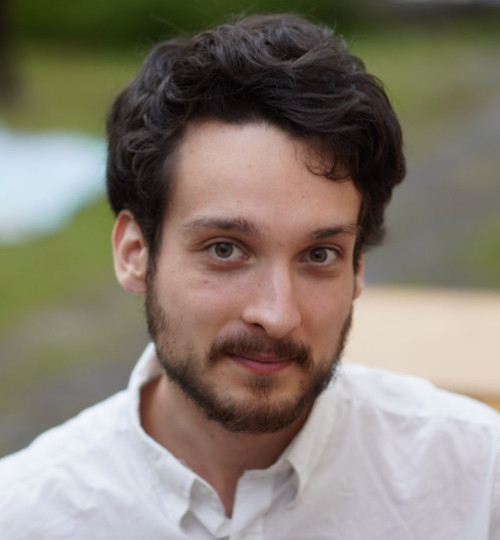
\includegraphics[width=3.85cm]{portrait.jpg}
%     \vspace{1cm}
% \end{minipage}

\hSectionI{Selected Academic Projects and Publications}{\href{https://scholar.google.com/citations?user=2EUDwtkAAAAJ}{Google Scholar}\hspace{-1.12cm}}

\hSubsectionB
{Neural Machine Translation Quality and Post-Editing Performance}
{\href{https://arxiv.org/pdf/2109.05016.pdf}{EMNLP 2021}}
{Vilém Zouhar, Ondřej Bojar, Martin Popel, Aleš Tamchyna}

\hSubsectionB
{Providing Backtranslation Improves Users Confidence in MT, Not Quality}
{\href{https://aclanthology.org/2021.naacl-main.14/}{NAACL 2021}}
{Vilém Zouhar, Michal Novák, Matúš Žilinec, Ondřej Bojar, Mateo Obregón, Robin L. Hill,\\ Frédéric Blain, Marina Fomicheva, Lucia Specia, Lisa Yankovskaya}
\vspace{-0.11cm}

\hSubsectionB
{Artefact Retrieval: Overview of NLP Models with Knowledge Base Access}
{\href{https://openreview.net/forum?id=9_oCNR6R9l2}{AKBC CSKB 2021}}
{Vilém Zouhar, Marius Mosbach, Debanjali Biswas, Dietrich Klakow}

\hSubsectionB
{Sampling and Filtering of Neural Machine Translation Distillation Data}
{\href{https://aclanthology.org/2021.naacl-srw.1/}{NAACL SRW 2021}}
{Vilém Zouhar}

\hSubsectionB
{Leveraging Neural Machine Translation for Word Alignment}
{\href{https://ufal.mff.cuni.cz/pbml/116/art-zouhar-pylypenko.pdf}{PBML 116}}
{Vilém Zouhar, Daria Pylypenko}

\hSubsectionB
{WMT20 Document-Level Markable Error Exploration}
{\href{https://aclanthology.org/2020.wmt-1.41/}{WMT20}}
{Vilém Zouhar, Tereza Vojtěchová, Ondřej Bojar}

\hSubsectionB
{Extending Ptakopět for MT User Interaction Experiments}
{\href{https://ufal.mff.cuni.cz/pbml/115/art-zouhar-novak.pdf}{PBML 115}}
{Vilém Zouhar, Michal Novák}

\hSubsectionB
{Outbound Translation User Interface Ptakopet: A Pilot Study}
{\href{https://aclanthology.org/2020.lrec-1.860/}{LREC 2020}}
{Vilém Zouhar, Ondřej Bojar}

\hSubsectionB
{A Collection of Machine Learning Excercises}
{2018/2019}
{
\hspace{-0.1cm}50 pages of ML tasks in R; full version available per request (used as \href{http://ufal.mff.cuni.cz/courses/npfl054}{teaching material}) \vspace{0.1cm}\newline
\vspace{-0.2cm}\hspace{-0.01cm}Awarded Student Faculty Grant at MFF Charles University
}

\hSubsectionB
{Paper on machine translation with eyetracking}
{in writing}
{Collaborator}

\hSubsectionB
{Paper on machine translation with EEG}
{in writing}
{Collaborator}

\hSubsectionB
{Paper on efficient knowledge base use}
{in writing}
{Main author}

\hSubsectionB
{Paper on partial answers as artefacts for classification}
{in writing}
{Main author}

\vspace{0.1\baselineskip}
\begin{minipage}{.62\textwidth}
    \hSection{Technical Knowledge}
    \hspace{-0.3cm}
    \begin{minipage}{\textwidth}
        \vspace{0.15cm}
        \begin{tabular}{ p{2.4cm} l}
        {\bf Programming} & Python, JS/TS, Rust, C/C++, R \\
        {\bf Toolkits} & PyTorch, Scikit, Marian NMT \\
        {\bf Misc.} & UNIX {\small (e.g. GPU cluster)}, Matplotlib, LaTeX \\
        & Always trying to learn more
        \end{tabular}
    \end{minipage}
\end{minipage}
\begin{minipage}{.38\textwidth}
    \hSection{Language Proficiency}
    \hspace{-0.3cm}
    \begin{minipage}{\textwidth}
        \vspace{0.15cm}
        \begin{tabular}{ p{1.3cm} l}
        {\bf Czech} & Native \\
        {\bf English} & C2 \textit{\footnotesize (iBT TOEFL 118/120)} \\
        {\bf German} & B2 \textit{\footnotesize (in development)} \\
        {\bf Polish} & A1
        \end{tabular}
    \end{minipage}
\end{minipage}

\newpage

\vspace{-0.1cm}
\hSection{Work Experience}
\hSubsectionItemize
{\href{https://www.lsv.uni-saarland.de/}{Spoken Language Systems} group (student research assistant)}
{(9 months) 2021}
{
    \item University of Saarland (Germany)
    \item Information retrieval efficiency through dimensionality reduction (\href{https://github.com/zouharvi/kb-shrink}{code})
    \item Language modelling with an external source of information
}

\hSubsection{Neural Networks Implementation and Application class (tutor)}{\footnotesize winter semester 2021 \hspace{-1.3cm}}
\vspace{-0.2cm}

\hSubsectionItemize
{Statistical Natural Language Processing class (tutor)}
{summer semester 2021}
{
    \item University of Saarland (Germany)
    \item Weekly tutorials for students
    \item Preparation of the \href{https://github.com/zouharvi/uds-snlp-tutorial}{SNLP class material}, \href{https://github.com/zouharvi/uds-nn-tutorial}{NN class material} and the final exam
    \item Designing and grading weekly assignments and the final project
    % \item Coordination among 2 other tutors
}

\hSubsectionItemize
{\href{https://ufal.mff.cuni.cz}{Institute of Formal and Applied Linguistics} (student research assistant)}
{2018-present}
{
    \item Charles Univeristy (Czech Republic)
    \item Machine translation related projects
    \item \href{https://browser.mt/}{Bergamot project} (in-browser MT)
    \item Psycholinguistic project consultation
    \item Miscellaneous research tasks
}

\hSubsectionItemize
{Previo (intern software dev)}
{(3 months) summer 2018}
{
    \item Development of multilayer CMS using JS, PHP, Zend and MySQL
}

\hSubsectionItemize
{BIM Project (intern software dev)}
{(3 months) summer 2017}
{
    \item Development of plugins for the ArchiCAD suite with C++/Boost and C\#
}

\hSubsectionItemize
{Web development}
{2015-2017}
{
\item Participation in several commercial website projects using the PHP/JS/HTML/CSS stack
\item Brno bez vizuálního smogu, MrFox, Velab, Intimedcare 
}


\hSection{Academic Misc.}

\hSubsectionItemize
{CSKB: Workshop on Commonsense Reasoning and Knowledge Bases}
{2022}
{
\item Organizational role to be determined
}


\hSubsectionItemize
{Department of Formal and Applied Linguistics}
{2019-present}
{
\item NER Presentation at NKÚ (supreme audit office)
\item Department presentation at Open Days
\item ELITR project coordination at a hackathon \href{https://elitr.eu/unihack-2020/}{UniHack}
}

\hSubsectionItemize
{Other projects}
{}
{
\item \href{https://github.com/zouharvi/multichannel-management}{Pandemic Crisis Communication}: Automatic Classification of Interviews With Experts \hfill {2021}
\item \href{https://github.com/zouharvi/user-models}{Fact Learning} with Adaptive Color Palette: Effect of Stimuli-Independent Hints \hfill {2021}
\item \href{https://github.com/zouharvi/rnn-bert-pos}{Hyperparameters of RNN Architectures}: for POS Tagging using Surface-Level BERT Embeddings \hfill {2021}
\item \href{https://github.com/zouharvi/deep-molecule-qspr}{Deep Molecule}: Quantitative Structure-Property Relationships \hfill {2021}
\item \href{https://github.com/zouharvi/SlowAlign}{SlowAlign}: 
IBM model-based word aligned with extra features and heuristics \hfill{2020}
\item \href{https://vilda.net/s/slowalign/}{SlowAlign Displayer}: Quick online word-alignment visualization tool \hfill {2020}
\item \href{https://github.com/zouharvi/MosQEto}{MosQEto}: Machine translation quality estimation data synthesis \hfill {2019}
\item Other small projects either for convenience, out of professional interest, or as a hobby, hosted at \href{https://github.com/zouharvi}{GitHub}
}



\hSection{Extra-Curricular}
\hSubsectionItemize
{Academic senate}
{2018-2020}
{
\item Member of the Academic Senate at Charles University Faculty of Mathematics and Physics
\item Participation in Faculty meetings, communicating with students, introductory summer camp 
}

\hSubsectionItemize
{Game Jams}
{2015-2020}
{
\item Several \href{https://github.com/allemansratten}{games} programmed and presented in limited time, mostly Ludum Dare
}

\hSubsectionItemize
{Kasiopea}
{2017-2019}
{
\item Organization of \href{https://kasiopea.matfyz.cz/}{Kasiopea}, an annual coding competition for talented high school students
}

\end{document}

